\documentclass{article}

\usepackage[T1]{fontenc}
\usepackage[spanish]{babel} %paquete para poner cosas en español
\usepackage{titling} %paquete para modificar el espaciado de los titulos
\usepackage[margin=.8in]{geometry} %paquete para poner márgenes más pequeños
\usepackage{titlesec} %paquete para modificar como se ven los titulos
\usepackage{graphicx} %paquete para meter imagenes
\usepackage{todonotes} %paquete para hacer \todo
\usepackage{pdfpages}
\usepackage{hyperref}
\hypersetup{ %Setup of hyperref package
	 colorlinks=true,
	 linkcolor=black,
	 filecolor=brown,		
	 urlcolor=blue,
	 pdftitle={TP5 Digitales},
	 }
\usepackage{minted}
\usepackage{float}

\graphicspath{{imagenes/}}

\titleformat{\section}
	{\bfseries \huge}
	{}
	{0em}
	{}[\titlerule]

\titleformat{\subsection}
	{\bfseries \Large}
	{}
	{0em}
	{}

\titleformat{\subsubsection}
	{\bfseries \large}
	{}
	{0em}
	{}

\titlespacing{\section} %me permite controlar el espaciado de la seccion que le indico
	{0em}
	{3em}
	{1.5em}

\newcommand{\sectionbreak}{\clearpage}
\renewcommand{\labelenumi}{\alph{enumi})}
%
%
%

\begin{document}
\begin{titlepage}
	 \begin{center}
		 \vspace*{1cm}
				
		 \Huge
		 \textbf{Trabajo Práctico Número 5}
				
		 \vspace{0.3cm}
		 \LARGE
		 Informe técnico	
		 
		 \vspace{0.5cm}
		 \Large
			Un trabajo presentado para la materia de \\
			Aplicaciones de electrónica digital
				
		 \vspace{1.5cm}
		\begin{figure}	[H]
		\centering
		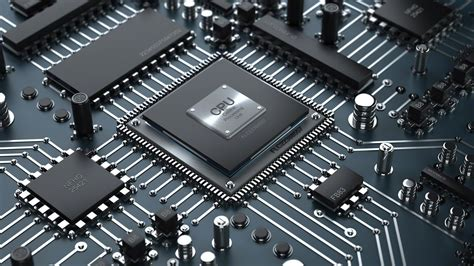
\includegraphics[width=0.6\textwidth]{logo}
		\end{figure}
		\vfill
		 \Large
		 \textbf{Krapp Ramiro -- Golmar Elias -- Pisacane Juan Cruz} \\
		 Instituto tecnológico San Bonifacio\\
		 Departamento de electrónica\\
		 \today
		 
		 \vspace{0.5cm}
		 \large {Hecho en \LaTeX}

	 \end{center}
\end{titlepage}

\setcounter{tocdepth}{3}
\tableofcontents
\noindent\rule{\textwidth}{0.7pt}

\section{Actividad}
	\subsection{Se pide:}
	\renewcommand{\labelenumi}{\alph{enumi})}
	\begin{enumerate}
		\item Dibujar circuito eléctrico. 
		\item Realizar diagrama de flujo. 
		\item Realizar código en lenguaje C. 
		\item Realizar bitácoras personales 
		\item Simular en PROTEUS. 
	\end{enumerate}
		
\section{Circuito Eléctrico}
Este es el circuito electrico:

\begin{figure}[H]
	\centering
	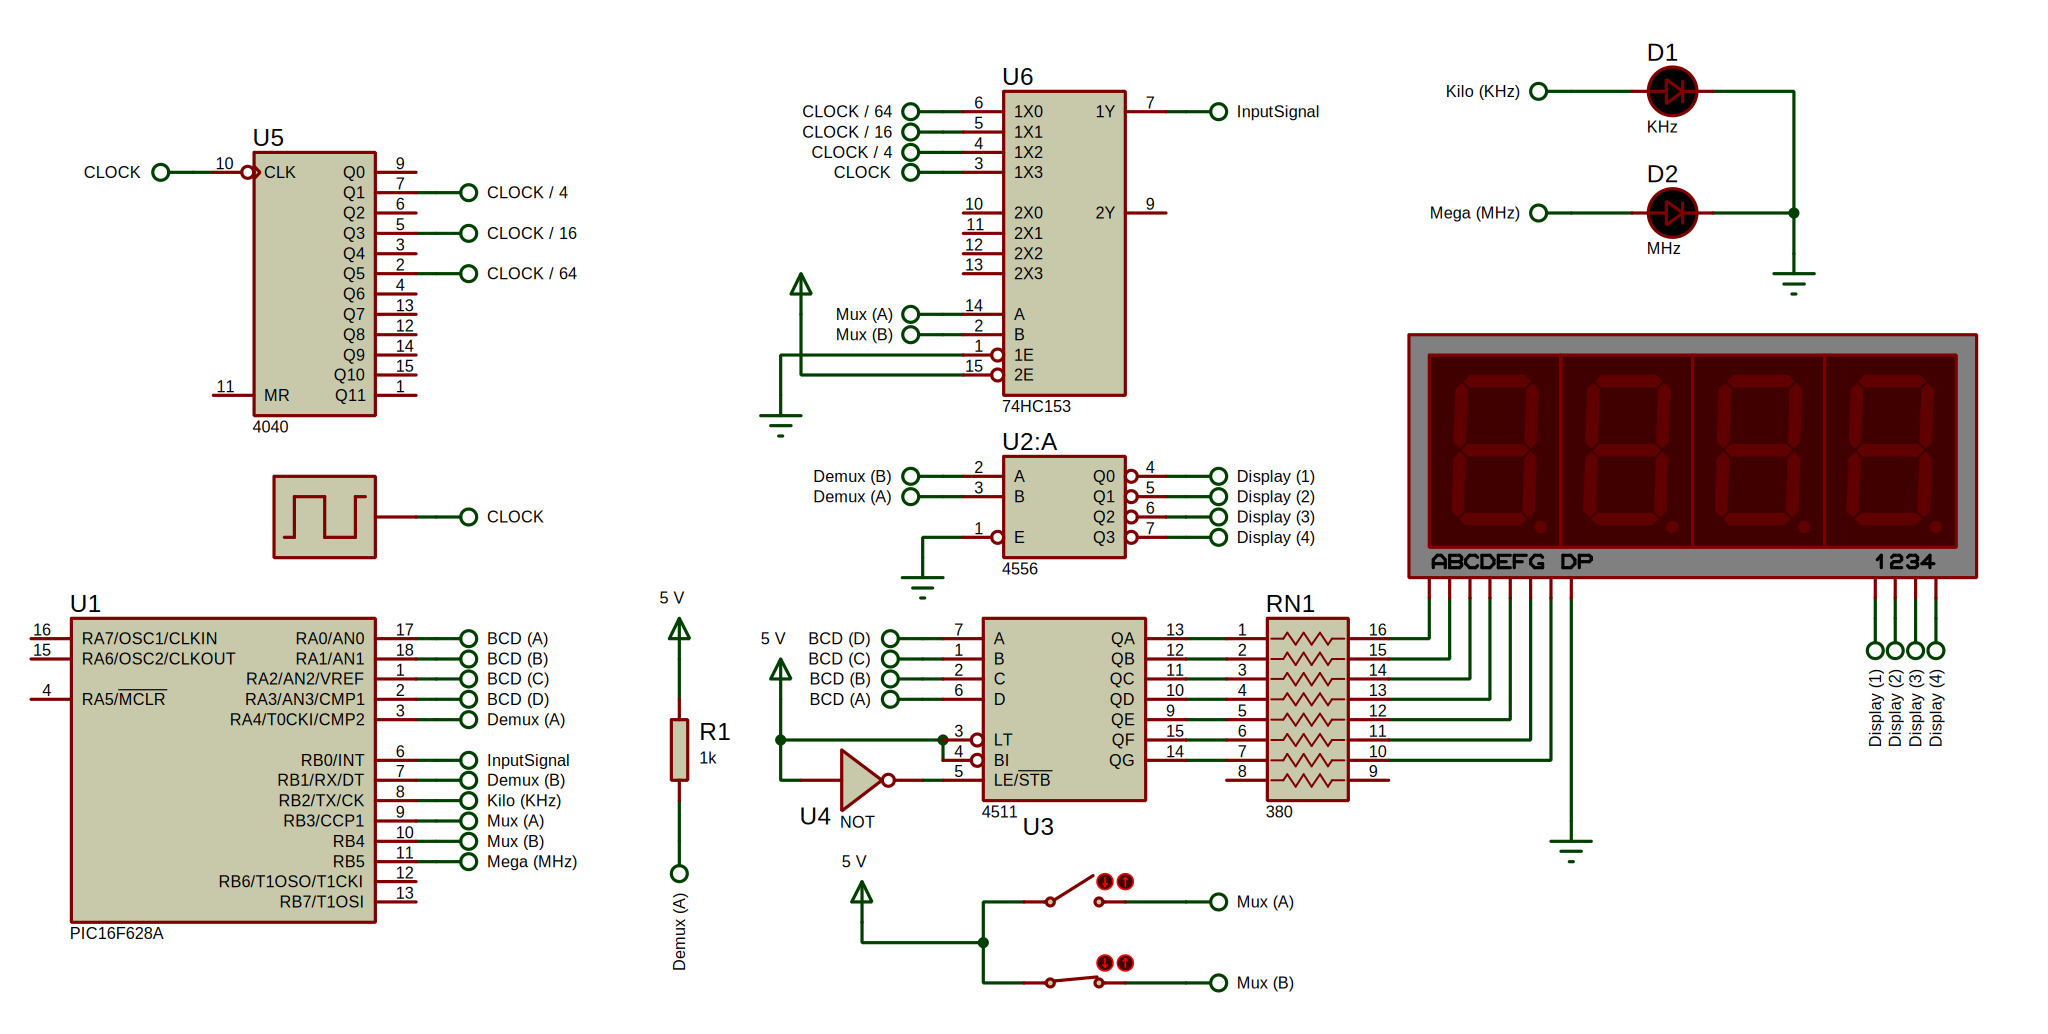
\includegraphics[width = \textwidth]{diagrama_esquematico}
	\caption{Diagrama esquematico hecho en Proteus}
\end{figure}

\section{Diagrama de flujo}
Este es el diagrama de flujo
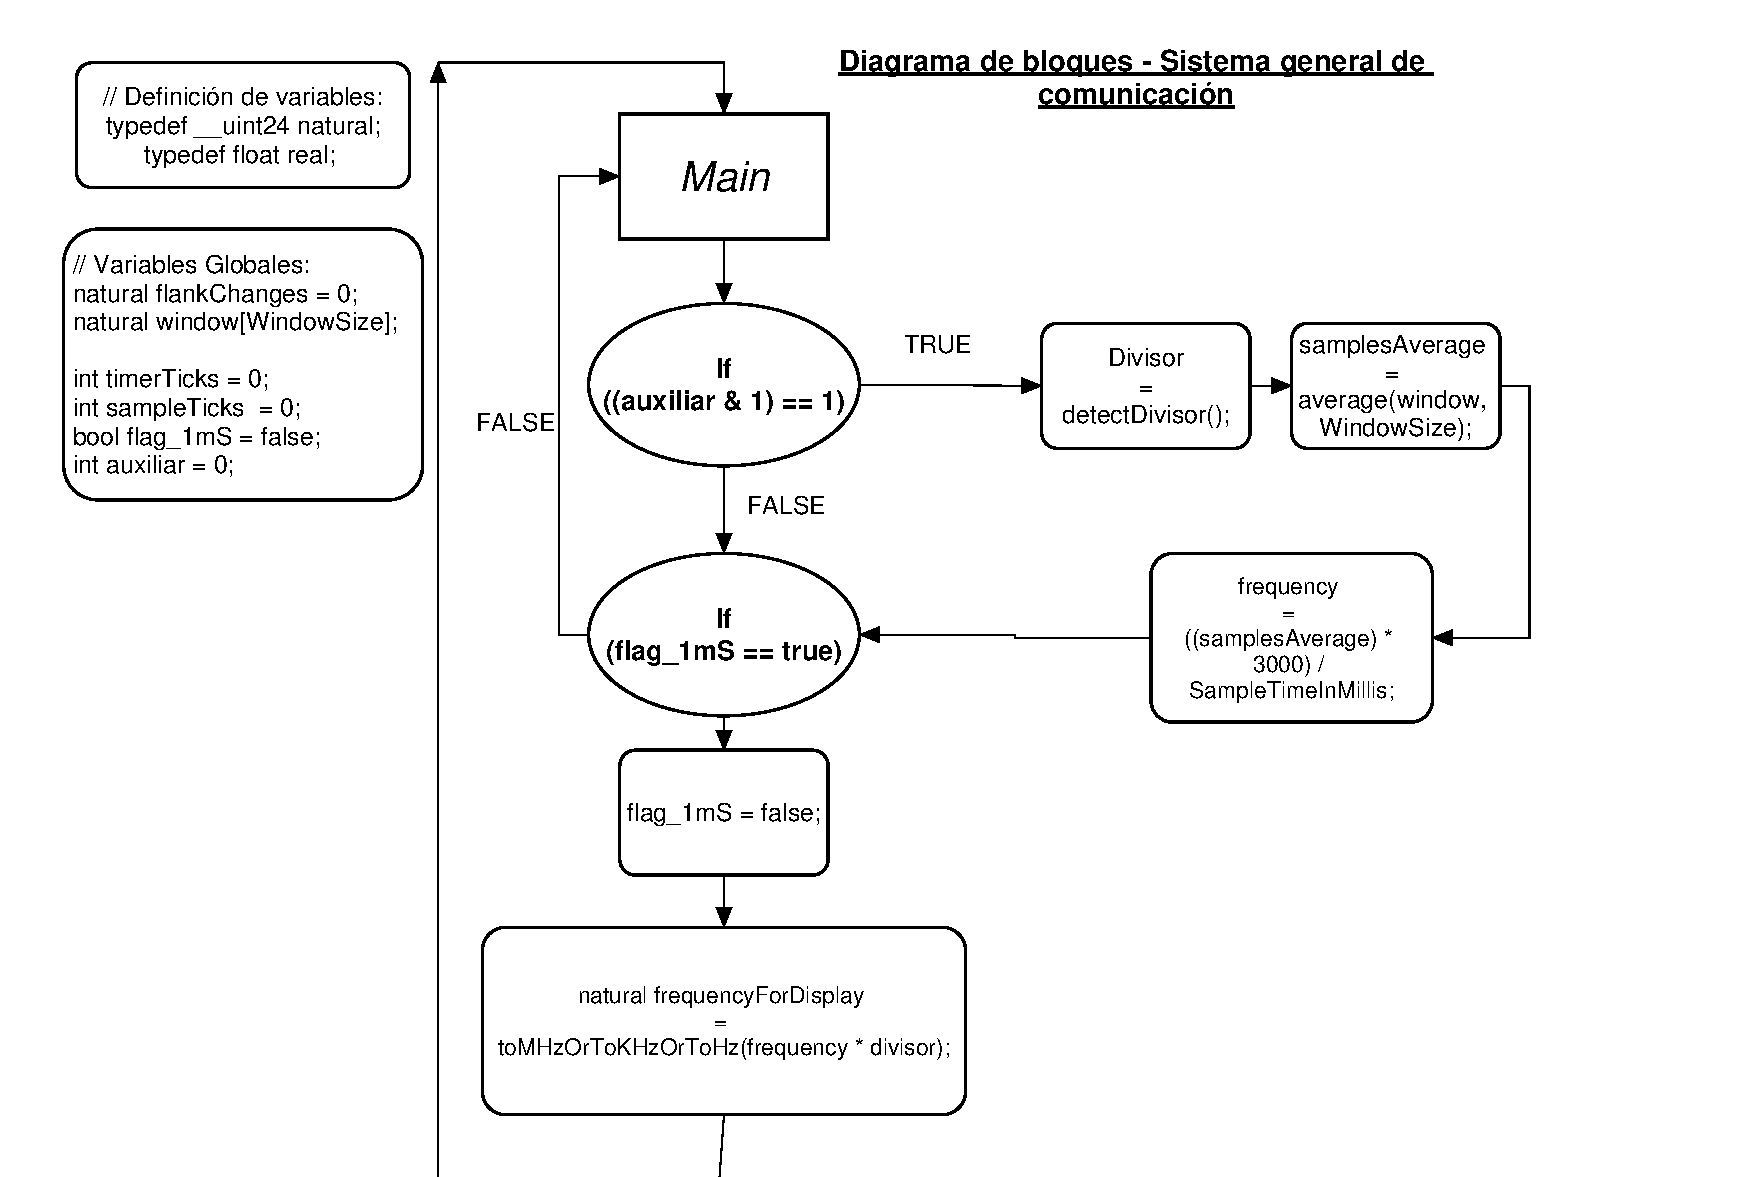
\includepdf[pages=-]{./imagenes/diagrama_flujo.pdf}
%\begin{figure}[H]
%	\centering
%	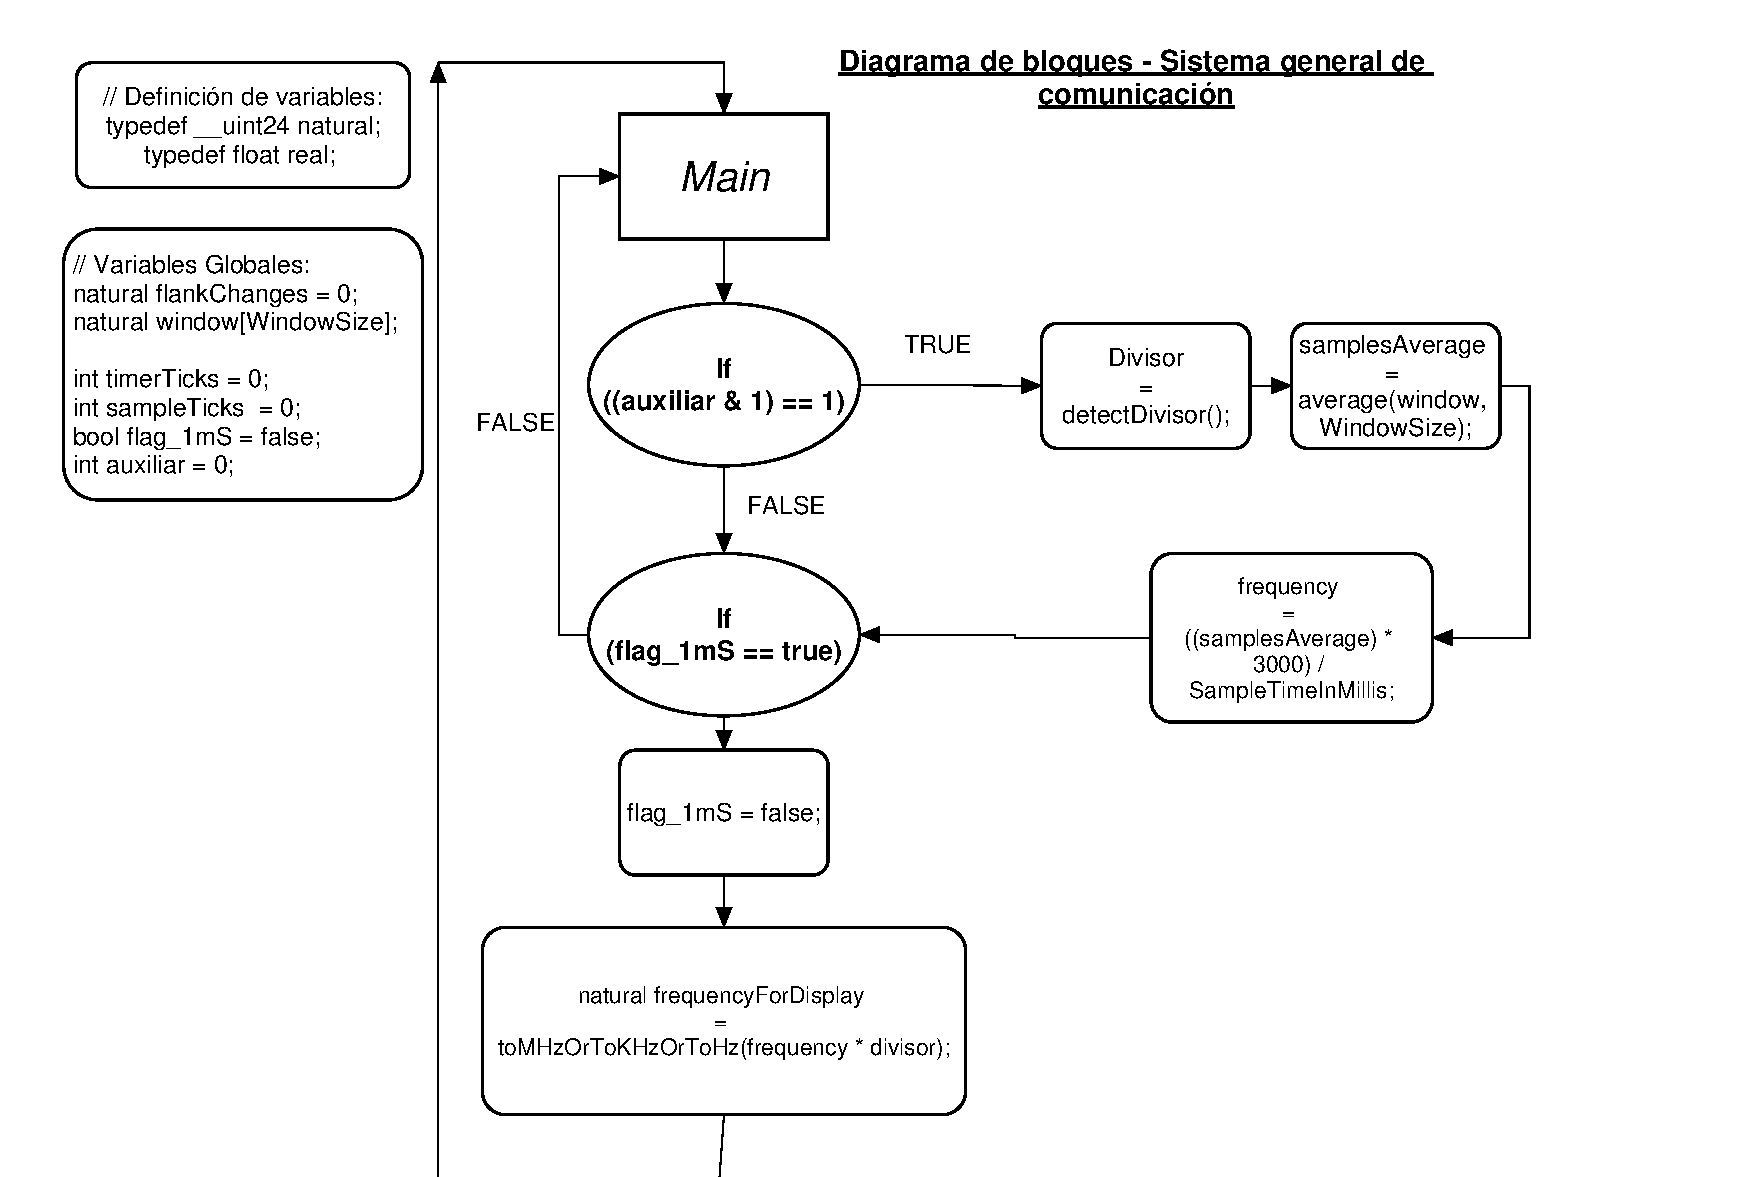
\includepdf[pages=-]{./imagenes/diagrama_flujo.pdf}
%	\caption{Flujo de C}
%\end{figure}

\section{Código en C}

\inputminted 
[frame= lines, linenos, breaklines, tabsize = 3, fontsize=\footnotesize, 
label=Codigo principal, fontseries=inconsolata]
{c}{./codigo/codigo_c.c}

\section{Bitacora}
Empezamos este código armando las funciones principales del proyecto.
Las funciones que nos resultaron más fundamentales fueron digitAt() y detectDivisor().
Tambien usamos typedef para definir nuestro propio tipo de dato.

Algo de lo que nos dimos cuenta fue de que a mayor cantidad de mediciones, mayor precisión
de la medición

\section{Simulaciones en Proteus}

	\subsection{C}
	\begin{itemize}
		\item \url{https://www.loom.com/share/27a263f557e74fb1976f201afc8397d8}
	\end{itemize}


\end{document}
